%\documentclass[prb.11pt,notitlepage]{revtex4-1}
%\documentclass[11pt,notitlepage]{revtex4-1}
\documentclass[11pt,a4paper]{article}
%---------------------------
% preambulo:
%---------------------------
\usepackage{abstract}
\usepackage[affil-it]{authblk}
\usepackage[utf8]{inputenc}	% encoding do arquivo, reconhecimento de acentos, etc.
\usepackage[brazilian]{babel}    % hiphenação em portugues
\usepackage{textcomp} % pacote para simbolos gregos no texto, sem ficar itálico
\usepackage{amsmath}    % need for subequations
\usepackage{amssymb}    % need for math symbols
\usepackage{graphicx}   % need for figures
\usepackage{verbatim}   % useful for program listings
\usepackage{color}      % use if color is used in text
\usepackage{subfigure}  % use for side-by-side figures
\usepackage{siunitx}
\usepackage{hyperref}   % use for hypertext links, including those to external documents and URLs
\usepackage[yyyymmdd,hhmmss]{datetime} % pacote para escrever a data de hoje
\usepackage[brazilian,nameinlink]{cleveref} % pacote para referenciar figuras e equacoes
\usepackage[table,xcdraw]{xcolor} % tabelas coloridas
\usepackage{circuitikz} %Pacote para desenhar circuitos
\usepackage{tikz}
\ctikzset{bipoles/length=0.9 cm} % tamanho dos componentes desenhados nos circuitos pelo pacote Circuitikz
\raggedbottom           % don't add extra vertical space
%---------------------------
%MARGENS
%---------------------------
\usepackage{indentfirst}        % indenta primeiro parágrafo
\setlength{\topmargin}{-15pt} % extra vert. space + at the top of header: 23pt
\setlength{\oddsidemargin}{-15pt} % extra spc added at the left of odd page: 0pt
\setlength{\textheight}{625pt} % comprimento do corpo do texto
\setlength{\textwidth}{480pt} % largura do corpo do texto
\setlength{\footskip}{50pt} % distancia da ultima linha de texto até número da pg.
%--------------------------
% INICIO DO DOCUMENTO:
%--------------------------
\begin{document}
%---------	
%cabeçalho
%---------
\title{Relatório 3: Transformadores\\
\small{F429 - G.5  2$^{ \underbar{\text{o}} }$ semestre 2016 \\
Prof. Lázaro Padilha }}
\author{Giovani Nascimento Pereira - 168609 \\
Seong Eun Kim - 177143\\
Renan Adriani Sterle - 176536\\
Carlos Augusto Figueiredo Freire de Carvalho - 165684}
\affil{ Universidade Estadual de Campinas \\ Faculdade de Engenharia Elétrica e Computação \\ Campinas, SP}

\date{\today}
%
% ======================================
% RESUMO
%
\maketitle
\begin{abstract}
    Nesse experimento, montamos um receptor de ondas AM e estudamos o papel de seus componentes. Para isso, montamos, inicialmente, circuitos para a caracterização de um filtro LC e da curva da corrente pela tensão do diodo. Assim, obtivemos a tensão de cotovelo $V_c \simeq 0.9285 V$, de forma que pudemos calcular a corrente de fuga $I_0 = 5.1203\cdot10^{-5} A$. Feito isso, construímos um circuito utilizando uma antena, um circuito ressonante como sintonizador, um diodo como demodulador e um alto-falante. A partir disso, pudemos compreender o funcionamento de um rádio galena, de transmissão em modulação AM, e explorar a relação entre a sintonização de frequências e o ajuste da capacitância do circuito ressonante.
    %
    %
    %%such dados, much resultados
    %
    %
    %
\end{abstract}

\newpage % nova pagina
\tableofcontents % cria sumário
%
% ======================================
% INTRODUCAO
%
\newpage
\section{Introdução}
    O experimento 4 - Diodo semicondutor e receptor AM, foi feito com o intuito de investigar a função dos componentes de um receptor de ondas AM e realizar sua montagem. Para isso, estudamos a atuação de um filtro ressonante sintonizável sobre a frequência e a tensão. Caracterizamos, também, a curva ixV de um diodo, de forma que pudemos obter a tensão de cotovelo, a partir da qual o diodo passa a conduzir corrente elétrica. Além disso, pudemos, por fim, aplicar os novos conhecimentos para ouvir a uma estação de rádio, utilizando, para isso, de uma antena, o filtro LC, o diodo como demodulador e um alto-falante.
    
\section{Objetivos}

    O experimento "Diodo semicondutor e Receptor AM teve como objetivo estudar e compreender o papel dos componentes de um Receptor de ondas AM no funcionamento durante a captação de ondas de rádio, através da caracterização da resposta em frequência de um circuito ressonante sintonizável, determinação da curva ixV de um diodo que permitiu a demodulação do sinal e com isso conseguir montar um circuito que permitia ouvir a uma emissora de rádio com modulação AM. Adotamos também o objetivo adicional de tentar sintonizar dois radiofaróis NDB de Campinas, CPN (515KHz) e IKP (370KHz), para ouvir o código Morse identificador.
    
\section{Metodologia}
    
    O experimento 4 permitiu estudar a transmissão de informação através de ondas eletromagnéticas. Para que uma transmissão desse tipo ocorra, o sinal da informação é codificado na onda portadora de forma a ser transmitido e recebido em outro lugar.
    
    A maneira de transmissão de informação através de uma onda eletromagnética varia de cada finalidade. Neste experimento estudamos mais a fundo as ondas de rádio AM (\textit{Amplitude Modulation}), onde a informação é adicionada a uma variação na amplitude da onda, a modulação, com frequencia bem menor à da onda portadora. No caso de ondas de rádio, essa modulação segue a forma da onda sonora codificada na onda eletromagnética. Um exemplo de modulação de ondas AM pode ser observada na \cref{OndasAM}.
    
        \begin{figure}[!htb]
        \centering
        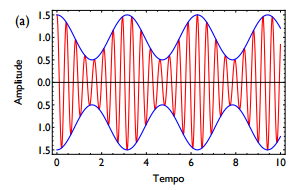
\includegraphics[scale=0.7]{OndasAM.png}
        \caption{Esquematização de uma onda de rádio AM, onde a frequência fica constante e a onda é modulada por um sinal}
        \label{OndasAM}
        \end{figure}
        
    Uma onda com modulacão AM \cite{livro2} pode ser descrita através da equação :
    
    \begin{equation}
        V = (1+ \delta (t))V_0cos(\omega t)
        \label{eqOndaAM}
    \end{equation}
    
    Onde $\omega t$ fazem referência a características da onda portadora, e sua frequência de transmissão, já o $\delta (t)$ representa a modulacão da amplitude da onda que carrega a informacão sonora.
    
    O circuito do Receptor utilizado pode ser observado na \cref{Receptor}. A primeira parte destacada em pontilhados na \cref{Receptor} descreve um filtro ressonante, constituído por um circuito LC em paralelo com um capacitor variável. Isso é importante para a montagem do receptor de rádio pois existem passando pelo local do experimento muitas frequências de ondas de rádio, ou outras ondas eletromagnéticas, e elas serão captadas pela antena do circuito. A fim de observar (ouvir) uma estação de rádio específica, é necessário filtrar essas ondas de rádio apenas na banda desejada.
    O filtro ressonante então funciona como um passa-banda, permitindo passar apenas as faixas próximas da estacão de interesse (com frequências próximas).
    
        \begin{figure}[!htb]
        \centering
        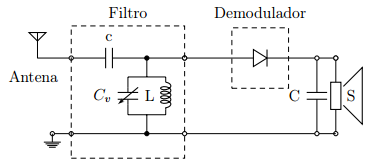
\includegraphics[scale=0.7]{Receptor.png}
        \caption{Circuito do Receptor AM montado. A primeira parte destacada refere-se ao filtro ressonante utilizado para filtragem das frequências recebidas pela antena, e a segunda parte destacada está diodo que funciona como o demodulador}
        \label{Receptor}
        \end{figure}
    
    O papel da antena acoplada ao circuito é transformar os sinais eletromagnéticos que incidem na mesma em sinais elétricos para o circuto. Quando uma onda eletromagnética, com frequência $f_c$ e comprimento
    de onda $\delta = c/f_c$, incide sobre uma antena, um dipolo oscilante é induzido na antena, que
    induz uma corrente no circuito no qual ela está conectada.
    
    Então, para o estudo do circuito, foi feita a montagem do circuito LC da \cref{Receptor}, conforme descrito na \cref{FiltroLC}.
    
        \begin{figure}[!htb]
        \centering
        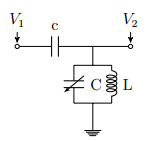
\includegraphics[scale=0.7]{FiltroLC.png}
        \caption{Circuito para caracterização do Filtro LC do Receptor AM da \cref{Receptor}}
        \label{FiltroLC}
        \end{figure}
    
    O filtro ressonante foi fornecido pronto constituído por um capacitor variável já ligado a um indutor e outro capacitor constante. Esse circuito todo foi ligado à alimentação através do gerador de função a uma frequência de $200KHz$ numa onda senoidal e a entrada e saída ligados ao osciloscópio para observação. Depois, com o auxílio do MatLAB e com o osciloscópio e o gerador de função ligados ao computador, foi feita uma varredura a fim de caracterizar a transmitância do filtro.
    
    A função resposta do filtro pode ser descrita como:
    
        \begin{equation}
            H(\omega) = \dfrac{X_C X_L}{X_cX_C + (X_c X_C)X_L} = \dfrac{\omega ^2 Lc}{\omega ^2L(C + c)-1}
            \label{eqTransmitanciaFiltroLC}
        \end{equation}
        
    A partir dessa equação é possível depreender que o circuito possui uma situação de ressonância $\omega _0$ em:
    
        \begin{equation}
            \omega _0 = \dfrac{1}{\sqrt{L(C+c)}}
            \label{eqRessonancia}
        \end{equation}
        
    Pois $H(\omega _0) \rightarrow \infty$. Mas isso ocorre pois consideramos o indutor ideal, sem resistência. Adicionando o valor da resistência do indutor (r), é possível obter a expressão para a transmitância do circuito como:
    
        \begin{equation}
            T(\omega _0) = c^2 L^2 \omega _0 ^4(1+L^2 \omega_0 ^2/r^2)
        \end{equation}
    
    De forma que agora, a transmitância não explode em $\omega _0$, mas sim gera um pico na função. Ou seja, determina uma passagem de banda de frequência do circuito.
    
        \begin{figure}[!htb]
        \centering
        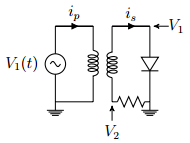
\includegraphics[scale=0.7]{CircDiodo.png}
        \caption{Circuito para caracterização da curva i-v do diodo}
        \label{CircDiodo}
        \end{figure}
        
    Com o filtro caracterizado, passamos para compreensão do decodificador, que é a segunda parte destacada na \cref{Receptor} e composta por um diodo. O circuito da \cref{CircDiodo} foi montado utilizando-se um transformador de isolação ($N_p = N_s$), ou seja, que não aumentava nem diminuía a tensão aplicada, para isolar os circuitos eletricamente, devido ao fato de os dois canais do osciloscópio terem um aterramento comum.
    
    Esse circuito permitia medir através do osciloscópio a tensão de alimentação do circuito, antes do diodo, ($V_1$), e a tensão de saída do diodo ($V_2$). Depois de montado, ele foi ligado ao osciloscópio para observação das formas de onda obtidas.
    Então, o oscilocópio foi ligado no modo XY para mostrar a curva i-v do diodo (É importante notar que se os canais forem invertidos, a curva mostrada nesta parte seria a curva v-i).
    
    Por fim, o circuito da \cref{Receptor} foi montado, utilizando o mesmo filtro da \cref{FiltroLC}, mas dessa vez com um diodo Schottky no lugar do demodulador (O motivo de usarmos este diodo, ao invés do diodo de silício, é que a tensão crítica na qual este diodo deixa passar corrente $(V_0 \approx 30 mV)$ é muito menor que o diodo de silício ($V_0 \simeq 700 mV$). Isto o torna ideal para demodular sinais de pequena amplitude, como o que recebemos da antena).
    
    A funcão do diodo pode ser descrita como:
    
        \begin{equation}
            I=I_0(e^{\beta v}-1)
            \label{eqDiodo}
        \end{equation}
    
    Sendo $I_0$ a corrente de fuga do diodo e $\beta = q/(TK_B)$ onde $K_B$ é a constante de Boltzmann e T é a temperatura do diodo.
    
    Sendo que, no cotovelo, a tensão pode ser aproximada por:
    
        \begin{equation}
            v_c \simeq -ln(I_0)/\beta
            \label{vc}
        \end{equation}
    
    E para situacoes próximas ao cotovelo do diodo, a equação pode ser aproximada por:
    
        \begin{equation}
            I(v) = av + bv^2
            \label{eqDiodoCotovelo}
        \end{equation}
    
    
    
    Quando colocamos a funcão de entrada proveniente da antena, e que passou pelo filtro do passa banda, ou seja, a \cref{eqOndaAM}, a onda é decomposta. Assumindo uma profundidade de modulacão baixa, $\delta$(t) $<<$ 1, as componentes podem ser descritas (simplificadamente) através da equação a seguir: 
    
        \begin{equation}
            I(t) = av(t) + bv(t) ^2 = Dc + A \delta (t)+B\delta (t)cos\omega t + C \delta(t) cos2\omega t
            \label{eqdecodificado}
        \end{equation}
        
    Onde DC é um fator constante, A, B e C são constantes também que dependem das propriedades do circuito. O importante é notar que após a demodulacão, um termo proporcional a $\cos\omega t$ surge, junto com um termo proporcional a $\cos2\omega t$ um termo constante (Dc) e uma oscilaćão proveniente da modulacão do sinal que é $\delta(t)$. Como esses sinais depois passam por um filtro passa baixa, e como as frequências de trasnmissão de onda de rádio são de frequência alta (da ordem de Mega Hertz), e a frequência da modulacão $\delta (t)$ representa a mesma frequência de ondas audíveis, ou seja, no intervalo de 20 a 20000 Hz,  apenas os termos Dc e A $\delta (t)$ \textit{passam} pelo filtro, sendo apenas o termo $A\delta (t)$ amplificado pelo amplificador e possível de ser ouvido.
    
    Depois, com o circuito montado, a capacitância variável do filtro ressonante foi variada até que fosse possível ouvir a  uma estação de rádio.
    
    
    %% ADICIONAR PARTE TEÓRICA DE CONTAS E TD MAIS
    
    
    Ao final do experimento, foi ligado o amplificador diretamente ao gerador de função, para que fosse possível ouvir as ondas geradas por ele. Foram colocadas várias formas de onda em várias frequências e com comportamentos distintos, mas apenas para observação. Testamos também os limites das faixas audíveis de frequência para humanos.
    
\newpage  
\section{Resultados}

    
        
    Ao montarmos o esquema representado na \cref{FiltroLC}, utilizando a capacitância mínima, fizemos a varredura da transmitância representada na \cref{Minima}.
    
        \begin{figure}[!htb]
        \centering
        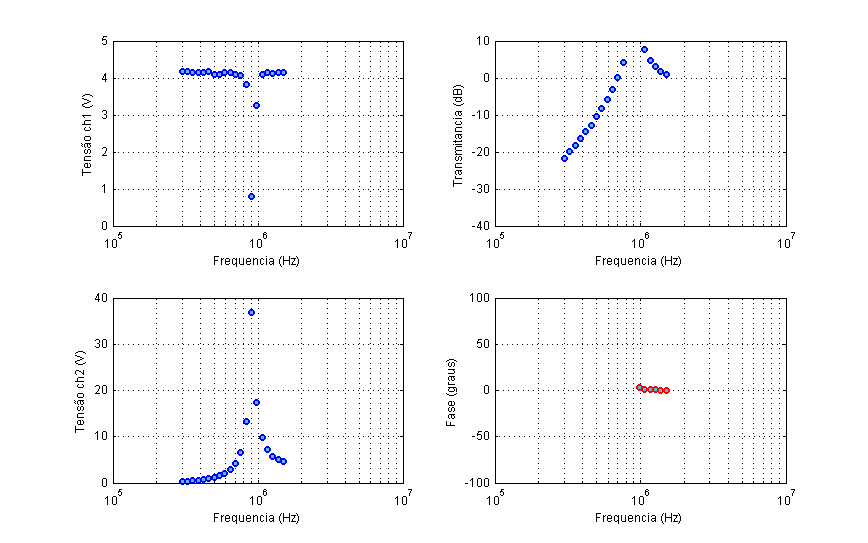
\includegraphics[scale=0.8]{TMinima.png}
        \caption{Imagem obtida através da varredura do osciloscópio para a trasmitância do filtro LC, descrito na \cref{FiltroLC}, com o capacitor colocado na capacitância mínima }
        \label{Minima}
        \end{figure}
    \newpage
    A partir do mesmo circuito, mas substituindo a capacitância mínima pela máxima, fizemos a varredura da transmitância do filtro ressonante LC, representada na \cref{TMaxima}.
    
        \begin{figure}[!htb]
        \centering
        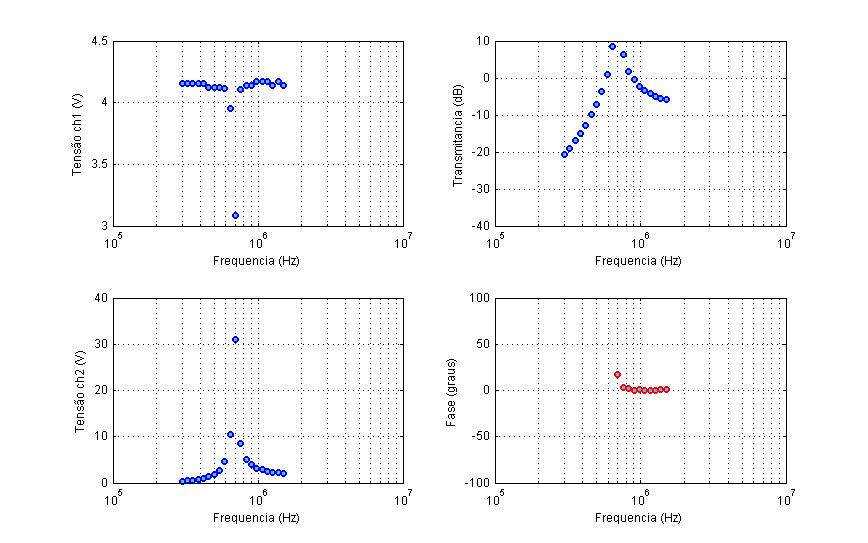
\includegraphics[scale=0.8]{TMaxima.png}
        \caption{Imagem obtida através da varredura do osciloscópio para a trasmitância do filtro LC, descrito na \cref{FiltroLC}, com o capacitor colocado na capacitância máxima }
        \label{TMaxima}
        \end{figure}
    
    Ao montarmos a \cref{CircDiodo}, pudemos fazer a varredura e obter as seguintes curvas:
    
        \begin{figure}[!htb]
        \centering
        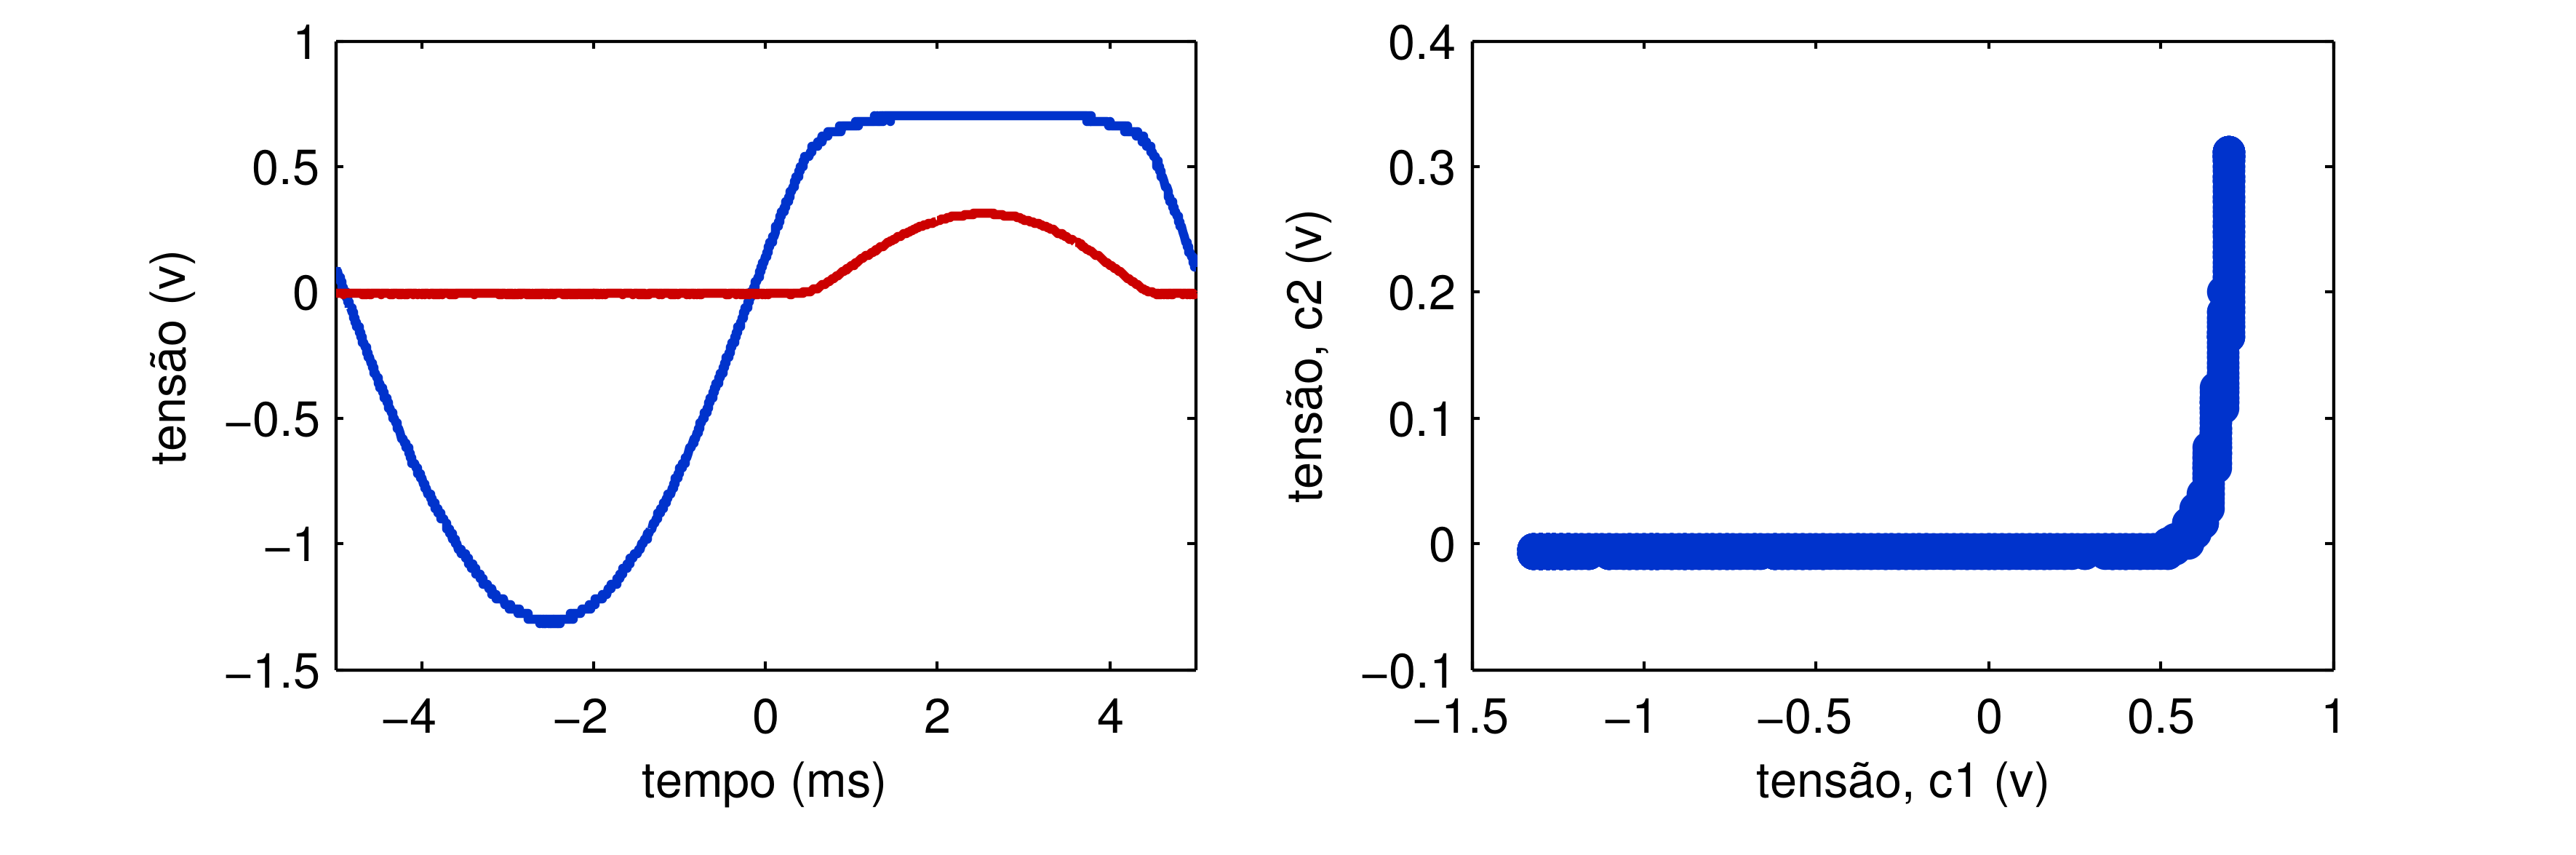
\includegraphics[scale=1]{CurvaDiodo.png}
        \caption{Imagem obtida através da varredura do osciloscópio para a curva da tensão no resistor pela tensão da fonte}
        \label{CurvaDiodo}
        \end{figure}
    
\section{Análise de Dados}

    Analisando as figuras \cref{Minima} e \cref{TMaxima}, especialmente quanto às transmitâncias, podemos notar claramente que a alteração na capacitância do circuito ressonante muda a frequência de ressonância, deslocando deslocando no eixo horizontal o pico da transmitância. Para sintonizar frequências mais altas, devemos utilizar capacitâncias menores, e vice-versa.

    Através dos dados obtidos da varredura feita com o auxílio do MATLab do comportamento do diodo, foi possível chegar na \cref{Grafico}.

        \begin{figure}[!htb]
        \centering
        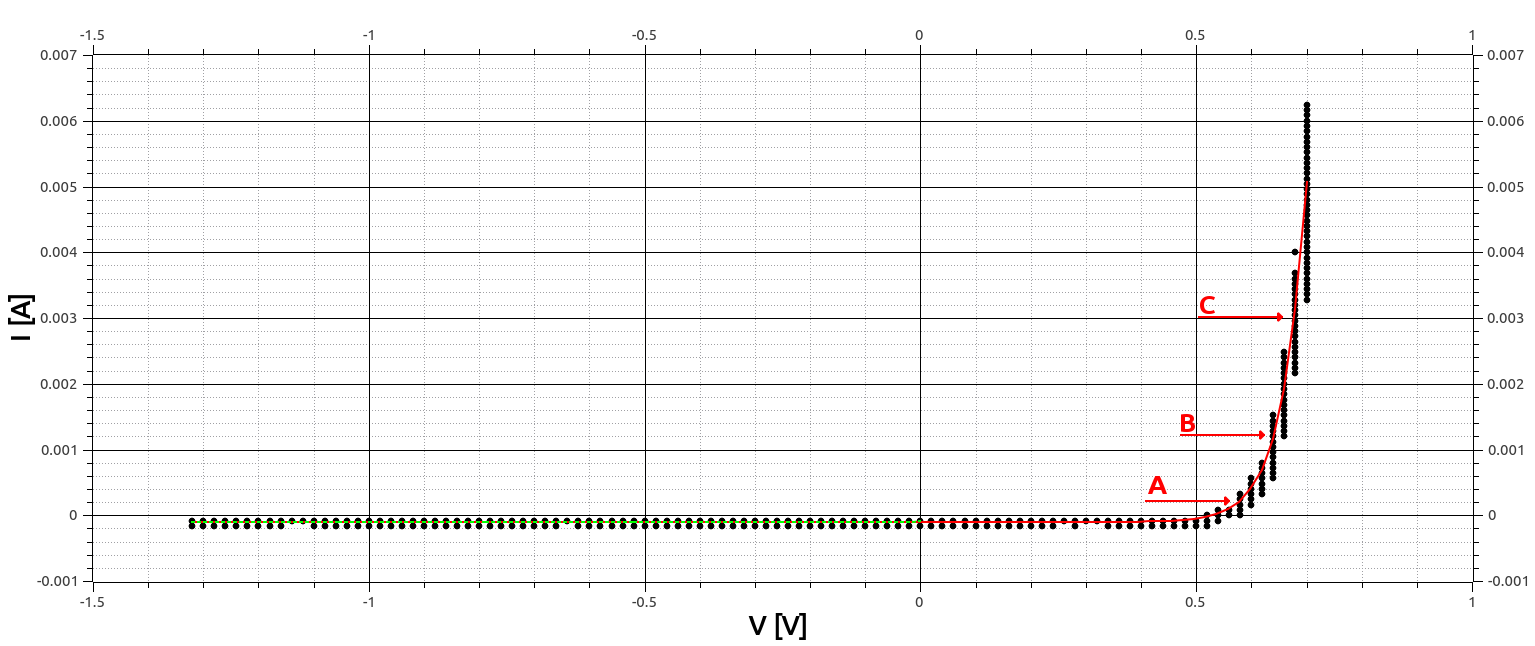
\includegraphics[scale=0.4]{Grafico.png}
        \caption{Gráfico i x V para o diodo de silício. A curva vermelha é a modelagem exponencial da corrente no diodo em todo o domínio ($I = I_0 (\exp(\beta V) - 1), I_0 = 5.1203\cdot10^{-5} A, \beta = 23.0391 \dfrac{1}{V}$). Em verde, a curva da corrente no diodo para a polaridade reversa. Os pontos A, B e C destacados são respectivamente (0.58, 0.00024), (0.64, 0.00120) e (0.68, 0.00304)}
        \label{Grafico}
        \end{figure}
        
    
    A curva obtida tem um comportamento exponencial, conforme previsto pela \cref{eqDiodo}. Através do gráfico, é possível obter os coeficiente $\beta$ e $I_0$ da equação. Infelizmente, o software utilizado para a modelagem (SciDAVis 1.D009) não nos forneceu corretamente os erros de $I_0$ e $B$. Ambos os valores de erros tiveram grandeza na ordem de $10^{-160}$, o que inviabilizou a propagação correta dos erros.
    
    Agora, com esses valores podemos estimar a tensão de cotovelo $V_c$ através da \cref{vc}, obtendo $V_c \simeq 0.9285 V$, que é próximo do valor esperado pela literatura $\simeq 0.7V$.
    
    Através do gráfico, pudemos modelar a curva do diodo para a polaridade reversa, e obter o coeficiente angular $M = (7 \pm 2)\cdot10^{-6}\dfrac{1}{\Omega}$ que está associado à corrente de fuga do diodo. De fato, o inverso deste coeficiente é a resistência equivalente do diodo para a polaridade invertida, sendo $R_d = (14 \pm 4)\cdot10^{4}\Omega$. Observamos que ela é muito grande.
    
    Com a modelagem exponencial para a corrente no sentido direto, pudemos determinar a resistência equivalente do diodo. Especificamente, para os três pontos A, B, e C indicados em \cref{Grafico}, calculamos a resistência através do inverso do coeficiente angular de $I(V)$ em cada ponto. Assim obtivemos $R_A = 133.3\Omega$, $R_B = 33.4\Omega$ e $R_C = 13.3\Omega$. Esses valores indicam que conforme a tensão aumenta e se afasta da tensão de cotovelo em sentido positivo, a resistência equivalente do diodo diminui.
    
    %PARTE 3!!!!!!!!!!
    Com o circuito da \cref{Receptor}, e conectado corretamente ao terra externo, foi possível sintonizar o circuito através da variação da capacitância do circuito, alterando a faixa de frequência que passava pelo filtro ressonante. Ao escutar a rádio sintonizada, foi possível descobrir que se tratava da Band AM, de frequência 1170 MHz.
    
    Nós alteramos também o capacitor fixo de modo a permitir sintonizar os radiofaróis CPN e IKP. No entanto, para nenhum deles conseguimos ouvir o código Morse identificador. Isso pode ter sido causado pela dificuldade em sintonizar as frequências, e também devido ao fato de a intensidade do sinal do sinal ser reduzida especialmente em virtude da altitude relativa ao solo, visto que os radiofaróis NDB não são otimizados para emissão a baixas altitudes.
    Por fim, o amplificador foi ligado diretamente ao gerador de função. Isso permite que ele transforme em ondas sonoras as formas de onda geradas pelo gerador, e assim foi possível ouvir o comportamento das ondas geradas, sonoramente, e averiguar que aumentando a frequência o som se tornava mais agudo, diminuindo mais grave, e os diferentes timbres gerados para cada função de onda diferente.


\section{Discussão}

    A curva obtida do diodo, teve a forma esperada de uma função exponencial \cite{livro}, que representa o comportamento desse componente eletrônico. A tensão de cotovelo encontrada foi de $V_c \simeq 0.9285 V$,  sendo que o valor esperado era de $0.7 V$ \cite{diodo}. É possível notar uma diferença entre os valores obtidos e o esperado pela literatura, mas isso provém possivelmente porque a expressão da tensão cotovelo do diodo utilizada é uma aproximação. 
    %DISCUSSAO DO ITEM 3 E 4
    Como conseguimos \textit{sintonizar} o circuito de forma a ouvir uma estacão de rádio (a Bandeirantes AM, na frequência de 1170 MHz), foi possível notar que o circuito se comportava como esperado. De todas as ondas eletromagnéticas incidentes na antena receptora, apenas essa foi filtrada e demodulada de forma a ser ouvida pelo amplificador. Tal limitação se deve ao fato de que o capacitor variável fornecido variava dentro de um intervalo limitado, restringindo, assim, o intervalo de frequências que poderiam passar pelo filtro ressonante e, assim, ser captadas.
    
    Isso demonstra tanto o funcionamento dos filtros que faziam parte do circuito, quanto o papel do demodulador.
    
    No final, quando escutamos o som gerado pelas funções do gerador de função, diretamente, foi possível notar que o amplificador apenas transforma em ondas sonoras a forma de onda da corrente que entra no circuito.
    
    Foi muito interessante testar os limites de audição das pessoas do laboratório, que fica realmente em torno de 20 a 20000 Hz, conforme o descrito para a literatura dos limites comuns da audição humana \cite{limiteAudicao}.
    
\section{Conclusão}


    Portanto podemos concluir que o circuito utilizado funciona como um receptor de ondas de rádio AM, já que foi possível utilizar o circuito para ouvir uma estação de rádio. Confirmamos que o filtro ressonante LC que tem a capacitância variável permite uma passagem de banda com uma frequência próxima ao desejado da \textit{sintonização} através da variação da capacitância do circuito. Foi possível confirmar o comportamento do diodo que retificava a onda, e permitia a passagem de tensão em apenas um sentido. Para o comportamento no \textit{cotovelo} do diodo, encontramos a tensão de cotovelo como sendo $V_c \simeq 0.9285 V$, através dos coeficientes da \cref{eqDiodo} sendo $\beta = 23.0391 \frac{1}{V}$ e a corrente de fuga $I_0 = 5.1203\cdot10^{-5} A$. Dessa forma, podemos concluir que o experimento cumpriu os seus objetivos e esteve de acordo com o esperado.


\section{Instrumentos utilizados}

    Os instrumentos utilizados neste experimento foram,
    \begin{itemize}
    	\item Osciloscópio Tektronix 10002B
    	\item Gerador de funções arbitrárias BK Instruments 4052
    	\item Multímetro DT830 Digital
    \end{itemize}


\begin{thebibliography}{10}
    
    \bibitem{apostila}Gustavo Wiederhecker e colaboradores, \textsl{Roteiros de F429 - Corrente alternada e óptica.} Compilado em 26 de setembro de 2016.
    
    \bibitem{livro texto}[Boyce and DiPrima, 2009 Boyce, W. E. and DiPrima, R. C. (2009)]. Elementary differential equations and boundary value problems. Wiley, Hoboken, NJ, 9th ed edition.
    
    \bibitem{livro}[Yaro Burian Jr. e Ana Cristina Lyra]. Circuitos Elétricos.
    
    \bibitem{livro2}Fundamentos da Física, Volume 3 - $9^a$edição.
    
    \bibitem{guia}[Gustavo S. Wiederhecker] Roteiros de F429 - Corrente alternada e óptica. 
    
    \bibitem{limiteAudicao} Human Audition Limits. Saiba mais sobre em:
    \url{https://en.wikipedia.org/wiki/Hearing_range}
    
    \bibitem{diodo} Diodos. Saiba mais em: \url{https://en.wikipedia.org/wiki/Diode}

\end{thebibliography}

\end{document}